\documentclass[../../lecture_notes.tex]{subfiles}

\begin{document}

\noindent We wish to learn both the parameters and structure of a Bayesian Network.

\subsection*{Parameters}
\noindent Consider the disease model from the previous lecture:

\begin{center}\begin{tikzpicture}
	\node [circle, draw, minimum height=1.5cm] (Co) {Cold};
	\node [circle, draw, right =of Co, minimum height=1.5cm] (Fl) {Flu};
	\node [circle, draw, right =of Fl, minimum height=1.5cm] (T) {Tonsilitis};
	\node [circle, draw, below left = of Fl, minimum height=1.5cm] (Ch) {Chill};
	\node [circle, draw, below right = of Fl, minimum height=1.5cm] (Fe) {Fever};
	\node [circle, draw, left =of Ch, align=center, minimum height=1.5cm] (ST) {Sore\\Throat};
	\node [circle, draw, right =of Fe, align=center, minimum height=1.5cm] (BA) {Body\\Ache};
	\draw [->] (Co.south) -- (ST.north east);
	\draw [->] (Co.south) -- (Ch.north);
	\draw [->] (Fl.south) -- (Ch.north);
	\draw [->] (Fl.south) -- (Fe.north);
	\draw [->] (T.south) -- (Fe.north);
	\draw [->] (T.south) -- (BA.north west);
	\draw [->] (Fl.south) -- (ST.north east);
	\draw [->] (Fl.south) -- (BA.north west);
\end{tikzpicture} \medskip

\begin{tabular} { | c | c c c c c c c | }\hline
	Case & Co & Fl & T & Ch & BA & ST & F\\\hline
	1 & T & F & ? & T & F & F & F\\
	2 & F & T & F & T & T & F & T\\ 
	3 & ? & ? & T & F & ? & T & F \\\hline
\end{tabular}\end{center}

\noindent Cases 1 and 3 have incomplete data, whereas 2 had \textbf{\underline{complete}}.\\
If every example is complete, the data set is called complete.\\
If complete, the maximum likelihood parameters are unique.\\
We find the likelihood of a parameter set like so:\\

\begin{minipage}{0.3\linewidth}
\begin{tabular} { | c | c c | } \hline
	F & A & $\theta$\\\hline
	T & T & $\theta_{A|F}$\\
	T & F & $\theta_{A|\neg F}$\\
	F & T & $\theta_{\neg A|F}$\\ 
	F & F & $\theta_{\neg A|\neg F}$\\\hline
\end{tabular}\end{minipage}%
\begin{minipage}{0.7\linewidth}
Param $\{S_1\} \rightarrow BN_1 \rightarrow Pr_1(.)$\\
Param $\{S_2\} \rightarrow BN_2 \rightarrow Pr_2(.)$\\
\indent .\\
\indent .\\
\indent .\\
We pick the set of parameters that maximizes the probability,\\
	\indent so score $S_i = \prod Pr_i (e_i)$ is the likelihood of parameters\\
\end{minipage}

\subsubsection*{Parameter Estimation With Complete Data}

\begin{center}\begin{minipage}{0.3\linewidth}\begin{tikzpicture}
	\node [circle, draw, minimum width =1.5cm] (H) {H};
	\node [circle, draw, below left =of H, minimum width =1.5cm] (S) {S};
	\node [circle, draw, below right =of H, minimum width =1.5cm] (E) {E};
	\draw[->] (H.south west) -- (S.north east);
	\draw[->] (H.south east) -- (E.north west);
\end{tikzpicture}\end{minipage}%
\begin{minipage}{0.7\linewidth}
\begin{center} \begin{minipage} {0.35\linewidth}
\begin{tabular}{ | c c c | c | }\hline 
	H & S & E & Pr(.)\\\hline 
	T & T & T & 2/16\\
	T & T & F & 0/16\\
	T & F & T & 9/16\\
	T & F & F & 1/16\\
	F & T & T & 0/16\\
	F & T & F & 1/16\\
	F & F & T & 2/16\\
	F & F & F & 1/16\\\hline
\end{tabular}\end{minipage}%
\begin{minipage}{0.35\linewidth}
\begin{tabular}{ | c | c | }\hline H & $\theta$\\\hline F & $\theta_h$\\T & $\theta_{\neg h}$\\\hline\end{tabular}\newline
\begin{tabular}{ | c | c | c | }\hline H & A & $\theta$\\\hline 
	T & T & $\theta{S|H}$\\
	T & F & $\theta{S|\neg H}$\\
	F & T & $\theta{\neg S|H}$\\ 
	F& F & $\theta{\neg S|\neg H}$\\\hline
\end{tabular}\end{minipage}\end{center}\end{minipage}\end{center}
\noindent The large table is our empirical distribution .\\
This is formed by collapsing our distribution:\begin{equation*}
	\theta_{\neg S|H} = \frac{Pr(\neg s,h)}{Pr(h)} = \frac{5}{6}\end{equation*}
This is our maximum likelihood parameter estimate!

\subsubsection*{Parameter Estimation With Incomplete Data}
\noindent This uses an iterative algorithm called \textbf{\underline{expected maximum}}.\\
Say we wish to fill the row <h, s, ?>.\\
We start with an arbitrary guess at the CPT.\\
	\indent $\text{CPT}_1 \rightarrow \text{ BN}_1 \rightarrow Pr_1(.)$.\\
We must choose from \{TFT, TFF\}, so we assign probabilities according to the probability function\\
	\indent x = Pr1(e|h, $\neg$s)\\
	\indent y = Pr($\neg$e|h, $\neg$s)\\
We then take the assignment with the greater probability, yielding\\
	\indent $\text{CPT}_2 \rightarrow \text{BN}_2 \rightarrow Pr_2(.)$.\\
\\
We only needed to surmise one term here, but we may need to iterate.\\
The probabilities Pr1(.) \& Pr2(.) are guaranteed to be non-increasing, so this converges.\\
This is thus a form of local search algorithm, so we know we may have to run repeatedly.\\
Note: this is the thinking behind the original algorithm, but it isn’t how it is performed in practice.\\

\subsection*{Structure}
\noindent Consider the following three structures:

\begin{center}\begin{minipage}{0.3\linewidth}\begin{tikzpicture} 
	\node[circle, draw] (B) {B};
	\node[circle, draw, below left =of B] (C) {C};
	\node[circle, draw, below right =of B] (D) {D};
	\node[circle, draw, below =of C] (A) {A};
	\draw [->] (B.south west) -- (C.north east);
	\draw [->] (B.south east) -- (D.north west);
	\draw [->] (C.south) -- (A.north);
\end{tikzpicture}\end{minipage}%
\begin{minipage}{0.3\linewidth}\begin{tikzpicture}
	\node[circle, draw] (B) {B};
	\node[circle, draw, below left =of B] (C) {C};
	\node[circle, draw, below right =of B] (D) {D};
	\node[circle, draw, below =of C] (A) {A};
	\draw [->] (B.south west) -- (C.north east);
	\draw [->] (B.south east) -- (D.north west);
	\draw [->] (C.south) -- (A.north);
	\draw [->] (D.south west) -- (A.north east);
\end{tikzpicture}\end{minipage}%
\begin{minipage}{0.3\linewidth}\begin{tikzpicture}
	\node[circle, draw] (B) {B};
	\node[circle, draw, below left =of B] (C) {C};
	\node[circle, draw, below right =of B] (D) {D};
	\node[circle, draw, below =of C] (A) {A};
	\draw [->] (B.south west) -- (C.north east);
	\draw [->] (B.south east) -- (D.north west);
	\draw [->] (C.south) -- (A.north);
	\draw [->] (D.south west) -- (A.east);
	\draw [->] (B.south) -- (A.north east);
	\draw [->] (D.west) -- (C.east);
\end{tikzpicture}\end{minipage}\end{center}

\noindent What do I need to optimize to choose between these three structures?\\
We have learned many of these algorithms, so we won’t discuss in detail, but:
	\begin{enumerate} [itemsep=0mm]
		\item local search methods ($\sim$ approximate methods)\\
				$\rightarrow$ we transform the structure looking for a better score\\
			We must thus specify movement within the neighborhood structure:\\
				$\rightarrow$ legal operations: add/remove/reverse edge
		\item systemic search methods ($\sim$ exact methods)\\
			$\rightarrow$ A* is a good example
	\end{enumerate} \medskip

\noindent Why can’t we just use maximum likelihood? We face \textbf{\underline{overfitting}}.\\
Say we are using likelihood to compare; then C > B > A.\\
	\indent We will thus end up with a complete DAG, no matter what.\\
	\indent Thus we need a model that balances structure complexity with likelihood.\\
	\indent Why? Consider:

\begin{center}
\begin{minipage}{0.2\textwidth}
	\begin{tabular} { | c | c | } \hline x & y\\\hline 1 & 1.1\\5 & 4.5\\10 & 11\\15 & 14.5\\20 & 22\\\hline\end{tabular}
\end{minipage}%
\begin{minipage}{0.8\textwidth}
	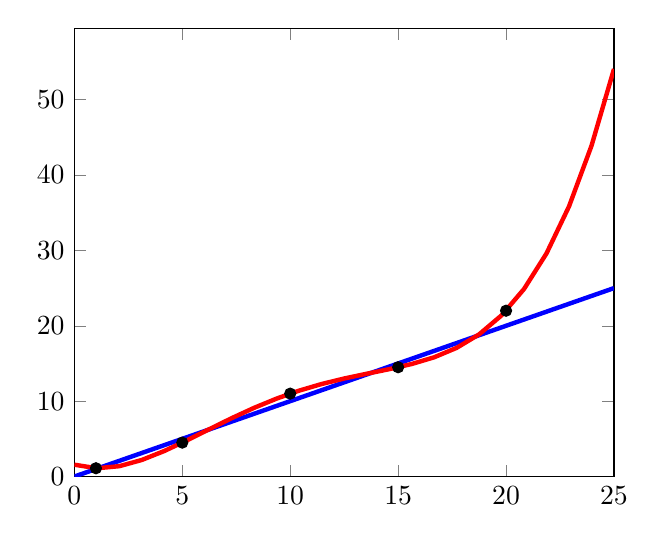
\begin{tikzpicture}
		\begin{axis} [xmin=0, xmax=25, ymin=0] (graph)
			
			\addplot[blue, ultra thick, domain=0:25] (x, x); 
			\addplot[red, ultra thick, domain=0:25] (x, 0.0009047619048*x*x*x*x 
											- 0.03590476191*x*x*x 
											+ 0.4516666667*x*x 
											- 0.8880952381*x 
											+ 1.571428572);
			\addplot [only marks] table {
			1 1.1
			5 4.5
			10 11
			15 14.5
			20 22
			};
		\end{axis}
	\end{tikzpicture}
\end{minipage}
\end{center}

\noindent The data is clearly a linear fit, but if we estimate to the fourth degree, we get bad data!\\
There is no fixed answer to the problem; \\
\indent we clearly need some function of the form f(likelihood) - g(complexity).\\
A common one is called MDK, but we need not discuss details.\\

\subsection*{Model-Oriented Vs. Query-Oriented Learning}
\noindent This can also be referred to as (unsupervised vs supervised) or (unlabeled vs labeled).\\
We have done model learning now; we move on to query based.\\
	\indent A model-based approach might give us the following:

\begin{center}\begin{minipage}{0.3\linewidth}
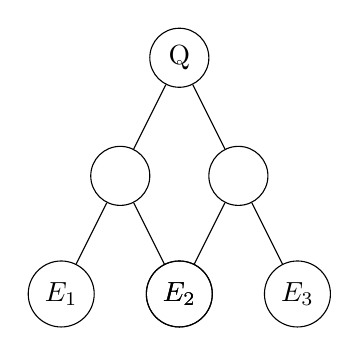
\begin{tikzpicture}
	\node [circle, draw, minimum size =0.75cm] {Q}
		child {node[circle, draw, minimum size =0.75cm] {}
			child {node[circle, draw, minimum size =0.75cm] {$E_1$}
				edge from parent}
			child {node[circle, draw, minimum size =0.75cm] {$E_2$}
				edge from parent} 
			edge from parent}
		child {node[circle, draw, minimum size =0.75cm] {}
			child {node[circle, draw, minimum size =0.75cm] {$E_2$}
				edge from parent}
			child {node[circle, draw, minimum size =0.75cm] {$E_3$}
				edge from parent} 
			edge from parent};
\end{tikzpicture}\end{minipage}%
\begin{minipage}{0.7\linewidth}
Currently we could give Q and ask for Pr($E_3$ or give $E_i$ and ask Pr(Q).\\
But we can improve performance by removing generality.\\
Say we promise only to infer upward:\\
Then we don’t ‘model’ the system and instead prepare for a specific ‘query’.\\
Labeling of correct responses is done by humans, and this is done to ‘train’.\\
If we want to talk about supervised learning, we need to introduce
\end{minipage}\end{center}

\subsubsection*{Arithmetic Circuits}

\begin{center}\begin{minipage}{0.65\linewidth}
\begin{figure}[H]
	\includegraphics[scale=0.15]{arithmetic_circuit}
\end{figure}\end{minipage}%
\begin{minipage}{0.36\linewidth}
\noindent The (+) symbols represent OR gates\\
The (*) symbols represent AND gates\\
The $\theta$ are the parameters\\
The $\lambda$ are the evidence\\
\end{minipage}\end{center}

When given a query, we can perform weighted model counting on the equivalent arithmetic circuit.\\
\indent If A=True, $\lambda_A = 1$; if A=False, $\lambda_{\neg A}$ = 1; if unknown, both are 1\\
Thus we can evaluate this in linear time;u nfortunately converting to an arithmetic circuit is $O(nd^w)$\\
\\
BUT what do we do if we don’t have the parameters?
We use the labeled data:

We want to set $\theta$ to maximize the chances of our data occurring.\\
We call this optimizing our \textit{loss function}.\\
Here, we often use cross \textbf{\underline{cross entropy}}\begin{equation*}
	<P(x), Q(x)> = \sum_x Q(x) log_2(P(x))\end{equation*}
Cross entropy gives us a measure of the disagreement between the two.\\
\indent Therefore, we often seek to minimize it across a structure.\\
We so this via gradient descent (nth dimensional hill climbing).\\

\begin{minipage}{0.3\linewidth}
\begin{center}\begin{tabular} { | c c c | }\hline A & C & B\\\hline T & T & F\\T & F & F\\. & . & .\\T & F & F\\\hline\end{tabular}\end{center}
\end{minipage}%
\begin{minipage}{0.7\linewidth}
We can feed \{A=T, C=T\} to the loss function. \\
Thus we get our 1-hot distribution for the missing variable(s):
\begin{center}\begin{tabular} { | c | c | }\hline B & Pr(B)\\T & 0\\F & 1\\\hline \end{tabular}\end{center}
\end{minipage}\medskip


\noindent Consider the example of recognizing shapes:
\begin{center}\begin{figure}[H]
	\includegraphics[scale=0.4]{rectangles}
\end{figure}\end{center}
\noindent Though pixel is functional in general, we allow it to be probabilistic to permit noise.\\
It will thus be inferred to be very close to 0/1.\\
A lot of heights will be zeroed as well depending on the column.\\
We can thus see that we have a lot of \textbf{\underline{background knowledge}}\\
\indent The simplest case of this is $A \iff B$, for which we could simply substitute and reduce cases.

\end{document}